\documentclass{standalone}
\usepackage{tikz}
\usetikzlibrary{patterns, positioning}
\usepackage[sfdefault]{ClearSans} %% option 'sfdefault' activates Clear Sans as the default text font
\usepackage[T1]{fontenc}

\begin{document}
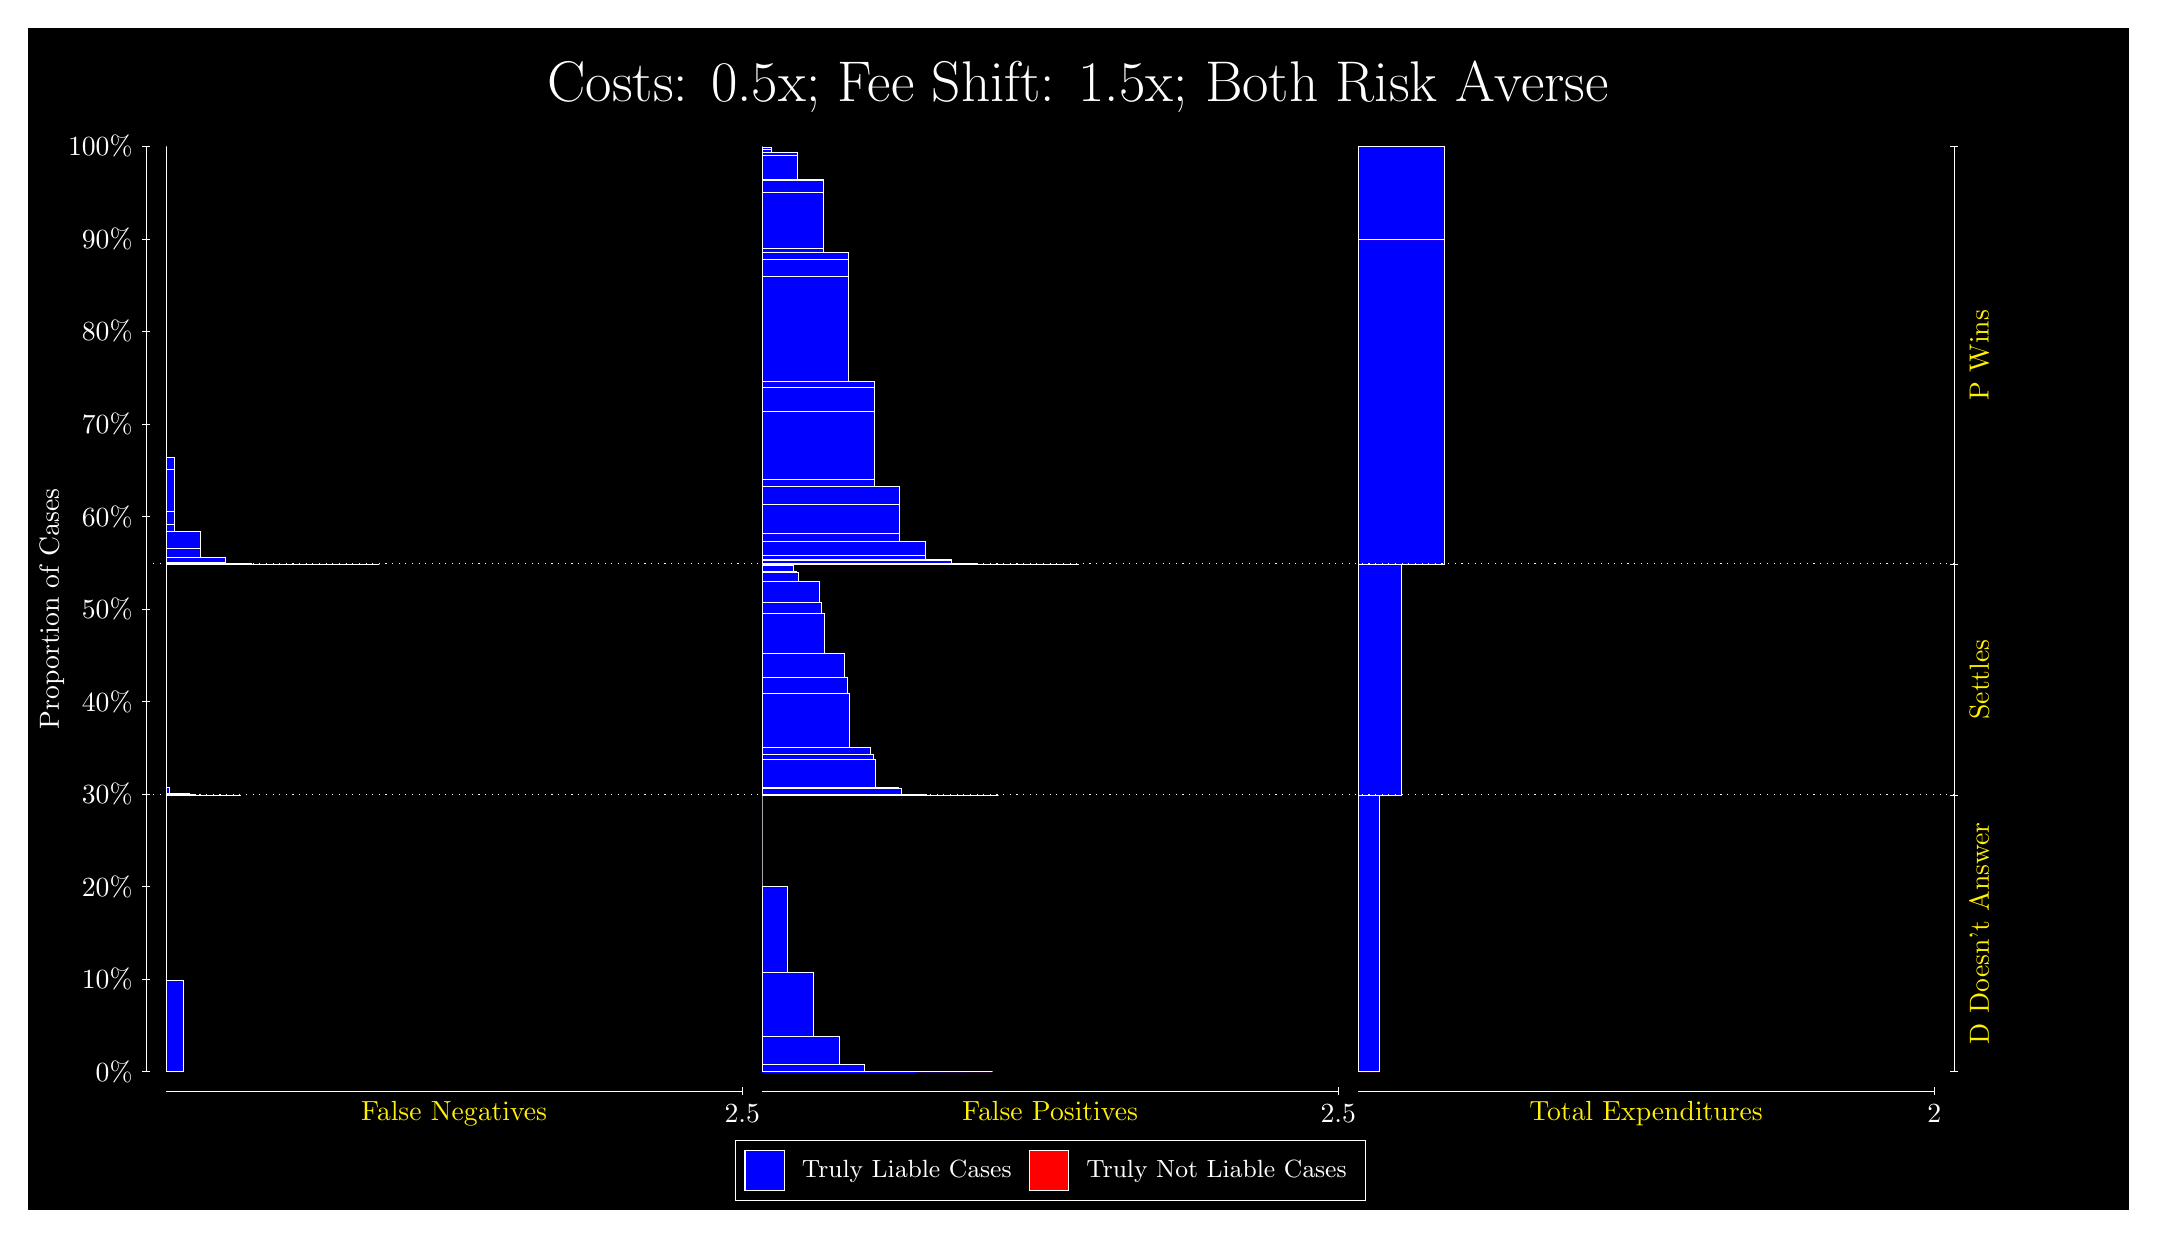
\begin{tikzpicture}
\draw[fill=black] (0,0) rectangle (26.667,15);
\draw[text=white] (0,13.5) rectangle (26.667,15) node[midway] {\huge Costs: 0.5x; Fee Shift: 1.5x; Both Risk Averse};
\draw[white, very thin] (1.5,1.75) -- (1.5,13.5);
\node[rotate=90, text=white, anchor=center] at (0.3, 7.625) {Proportion of Cases};
\draw[white, very thin] (1.45,1.75) -- (1.55,1.75);
\node[text=white, anchor=east] at (1.45, 1.75) {0\%};
\draw[white, very thin] (1.45,2.925) -- (1.55,2.925);
\node[text=white, anchor=east] at (1.45, 2.925) {10\%};
\draw[white, very thin] (1.45,4.1) -- (1.55,4.1);
\node[text=white, anchor=east] at (1.45, 4.1) {20\%};
\draw[white, very thin] (1.45,5.275) -- (1.55,5.275);
\node[text=white, anchor=east] at (1.45, 5.275) {30\%};
\draw[white, very thin] (1.45,6.45) -- (1.55,6.45);
\node[text=white, anchor=east] at (1.45, 6.45) {40\%};
\draw[white, very thin] (1.45,7.625) -- (1.55,7.625);
\node[text=white, anchor=east] at (1.45, 7.625) {50\%};
\draw[white, very thin] (1.45,8.8) -- (1.55,8.8);
\node[text=white, anchor=east] at (1.45, 8.8) {60\%};
\draw[white, very thin] (1.45,9.975) -- (1.55,9.975);
\node[text=white, anchor=east] at (1.45, 9.975) {70\%};
\draw[white, very thin] (1.45,11.15) -- (1.55,11.15);
\node[text=white, anchor=east] at (1.45, 11.15) {80\%};
\draw[white, very thin] (1.45,12.325) -- (1.55,12.325);
\node[text=white, anchor=east] at (1.45, 12.325) {90\%};
\draw[white, very thin] (1.45,13.5) -- (1.55,13.5);
\node[text=white, anchor=east] at (1.45, 13.5) {100\%};

\draw[white, very thin] (24.457,1.75) -- (24.457,13.5);
\draw[white, very thin] (24.407,1.75) -- (24.507,1.75);
\node[anchor=west] at (24.407, 1.75) {};
\draw[white, very thin] (24.407,5.264) -- (24.507,5.264);
\node[anchor=west] at (24.407, 5.264) {};
\draw[white, very thin] (24.407,8.1963) -- (24.507,8.1963);
\node[anchor=west] at (24.407, 8.1963) {};
\draw[white, very thin] (24.407,13.5) -- (24.507,13.5);
\node[anchor=west] at (24.407, 13.5) {};

\draw[white, very thin, fill=blue] (1.75,1.75) rectangle (1.9696,2.9145);
\draw[white, very thin, fill=red] (1.75,2.9145) rectangle (1.75,2.9145);
\draw[white, very thin, fill=blue] (1.75,2.9145) rectangle (1.75,5.264);
\draw[white, very thin, fill=blue] (1.75,5.264) rectangle (2.7015,5.264);
\draw[white, very thin, fill=blue] (1.75,5.264) rectangle (2.4087,5.264);
\draw[white, very thin, fill=blue] (1.75,5.264) rectangle (2.3762,5.2641);
\draw[white, very thin, fill=blue] (1.75,5.2641) rectangle (2.1159,5.2742);
\draw[white, very thin, fill=blue] (1.75,5.2742) rectangle (2.0834,5.2747);
\draw[white, very thin, fill=blue] (1.75,5.2747) rectangle (2.0509,5.28);
\draw[white, very thin, fill=blue] (1.75,5.28) rectangle (1.7907,5.3558);
\draw[white, very thin, fill=blue] (1.75,5.3558) rectangle (1.7581,5.375);
\draw[white, very thin, fill=red] (1.75,5.375) rectangle (1.75,5.375);
\draw[white, very thin, fill=blue] (1.75,5.375) rectangle (1.75,8.1963);
\draw[white, very thin, fill=blue] (1.75,8.1963) rectangle (4.458,8.1963);
\draw[white, very thin, fill=blue] (1.75,8.1963) rectangle (4.1327,8.1963);
\draw[white, very thin, fill=blue] (1.75,8.1963) rectangle (3.8074,8.1963);
\draw[white, very thin, fill=blue] (1.75,8.1963) rectangle (3.8074,8.1963);
\draw[white, very thin, fill=blue] (1.75,8.1963) rectangle (3.4821,8.1963);
\draw[white, very thin, fill=blue] (1.75,8.1963) rectangle (3.1568,8.1968);
\draw[white, very thin, fill=blue] (1.75,8.1968) rectangle (3.1568,8.1971);
\draw[white, very thin, fill=blue] (1.75,8.1971) rectangle (2.8316,8.2061);
\draw[white, very thin, fill=blue] (1.75,8.2061) rectangle (2.5063,8.2207);
\draw[white, very thin, fill=blue] (1.75,8.2207) rectangle (2.5063,8.2776);
\draw[white, very thin, fill=blue] (1.75,8.2776) rectangle (2.181,8.3951);
\draw[white, very thin, fill=blue] (1.75,8.3951) rectangle (2.181,8.614);
\draw[white, very thin, fill=blue] (1.75,8.614) rectangle (1.8557,8.6948);
\draw[white, very thin, fill=blue] (1.75,8.6948) rectangle (1.8557,8.8682);
\draw[white, very thin, fill=blue] (1.75,8.8682) rectangle (1.8557,9.4032);
\draw[white, very thin, fill=blue] (1.75,9.4032) rectangle (1.8557,9.5459);
\draw[white, very thin, fill=red] (1.75,9.5459) rectangle (1.75,9.5459);
\draw[white, very thin, fill=blue] (1.75,9.5459) rectangle (1.75,13.5);
\draw[white, very thin, fill=red] (9.3189,1.75) rectangle (12.246,1.75);
\draw[white, very thin, fill=blue] (9.3189,1.75) rectangle (12.246,1.75);
\draw[white, very thin, fill=blue] (9.3189,1.75) rectangle (11.921,1.75);
\draw[white, very thin, fill=blue] (9.3189,1.75) rectangle (11.596,1.75);
\draw[white, very thin, fill=blue] (9.3189,1.75) rectangle (11.271,1.7503);
\draw[white, very thin, fill=blue] (9.3189,1.7503) rectangle (10.945,1.7576);
\draw[white, very thin, fill=blue] (9.3189,1.7576) rectangle (10.62,1.8361);
\draw[white, very thin, fill=blue] (9.3189,1.8361) rectangle (10.295,2.1984);
\draw[white, very thin, fill=blue] (9.3189,2.1984) rectangle (9.9694,3.0086);
\draw[white, very thin, fill=blue] (9.3189,3.0086) rectangle (9.6442,4.0995);
\draw[white, very thin, fill=blue] (9.3189,4.0995) rectangle (9.3189,5.264);
\draw[white, very thin, fill=red] (9.3189,5.264) rectangle (12.32,5.264);
\draw[white, very thin, fill=blue] (9.3189,5.264) rectangle (12.32,5.264);
\draw[white, very thin, fill=red] (9.3189,5.264) rectangle (12.027,5.264);
\draw[white, very thin, fill=blue] (9.3189,5.264) rectangle (12.027,5.264);
\draw[white, very thin, fill=blue] (9.3189,5.264) rectangle (11.994,5.264);
\draw[white, very thin, fill=red] (9.3189,5.264) rectangle (11.734,5.264);
\draw[white, very thin, fill=blue] (9.3189,5.264) rectangle (11.734,5.2644);
\draw[white, very thin, fill=blue] (9.3189,5.2644) rectangle (11.702,5.2644);
\draw[white, very thin, fill=blue] (9.3189,5.2644) rectangle (11.669,5.2644);
\draw[white, very thin, fill=blue] (9.3189,5.2644) rectangle (11.409,5.2722);
\draw[white, very thin, fill=blue] (9.3189,5.2722) rectangle (11.376,5.2725);
\draw[white, very thin, fill=blue] (9.3189,5.2725) rectangle (11.344,5.2725);
\draw[white, very thin, fill=blue] (9.3189,5.2725) rectangle (11.084,5.3512);
\draw[white, very thin, fill=blue] (9.3189,5.3512) rectangle (11.051,5.3582);
\draw[white, very thin, fill=blue] (9.3189,5.3582) rectangle (11.018,5.3629);
\draw[white, very thin, fill=blue] (9.3189,5.3629) rectangle (10.758,5.7161);
\draw[white, very thin, fill=blue] (9.3189,5.7161) rectangle (10.726,5.7825);
\draw[white, very thin, fill=blue] (9.3189,5.7825) rectangle (10.693,5.8701);
\draw[white, very thin, fill=blue] (9.3189,5.8701) rectangle (10.433,6.5551);
\draw[white, very thin, fill=blue] (9.3189,6.5551) rectangle (10.4,6.7515);
\draw[white, very thin, fill=blue] (9.3189,6.7515) rectangle (10.368,7.0626);
\draw[white, very thin, fill=blue] (9.3189,7.0626) rectangle (10.108,7.5701);
\draw[white, very thin, fill=blue] (9.3189,7.5701) rectangle (10.075,7.709);
\draw[white, very thin, fill=blue] (9.3189,7.709) rectangle (10.043,7.9756);
\draw[white, very thin, fill=blue] (9.3189,7.9756) rectangle (9.7824,8.0853);
\draw[white, very thin, fill=blue] (9.3189,8.0853) rectangle (9.7499,8.1045);
\draw[white, very thin, fill=blue] (9.3189,8.1045) rectangle (9.7173,8.1803);
\draw[white, very thin, fill=blue] (9.3189,8.1803) rectangle (9.4571,8.1856);
\draw[white, very thin, fill=blue] (9.3189,8.1856) rectangle (9.4246,8.1861);
\draw[white, very thin, fill=blue] (9.3189,8.1861) rectangle (9.3921,8.1962);
\draw[white, very thin, fill=blue] (9.3189,8.1962) rectangle (9.3189,8.1963);
\draw[white, very thin, fill=red] (9.3189,8.1963) rectangle (13.344,8.1963);
\draw[white, very thin, fill=blue] (9.3189,8.1963) rectangle (13.344,8.1963);
\draw[white, very thin, fill=red] (9.3189,8.1963) rectangle (13.019,8.1963);
\draw[white, very thin, fill=blue] (9.3189,8.1963) rectangle (13.019,8.1963);
\draw[white, very thin, fill=red] (9.3189,8.1963) rectangle (12.694,8.1963);
\draw[white, very thin, fill=blue] (9.3189,8.1963) rectangle (12.694,8.1963);
\draw[white, very thin, fill=blue] (9.3189,8.1963) rectangle (12.368,8.1964);
\draw[white, very thin, fill=red] (9.3189,8.1964) rectangle (12.368,8.1964);
\draw[white, very thin, fill=blue] (9.3189,8.1964) rectangle (12.368,8.1969);
\draw[white, very thin, fill=red] (9.3189,8.1969) rectangle (12.043,8.1969);
\draw[white, very thin, fill=blue] (9.3189,8.1969) rectangle (12.043,8.2007);
\draw[white, very thin, fill=blue] (9.3189,8.2007) rectangle (12.043,8.2021);
\draw[white, very thin, fill=blue] (9.3189,8.2021) rectangle (12.043,8.2038);
\draw[white, very thin, fill=red] (9.3189,8.2038) rectangle (11.718,8.2038);
\draw[white, very thin, fill=blue] (9.3189,8.2038) rectangle (11.718,8.2444);
\draw[white, very thin, fill=blue] (9.3189,8.2444) rectangle (11.718,8.2541);
\draw[white, very thin, fill=blue] (9.3189,8.2541) rectangle (11.393,8.3075);
\draw[white, very thin, fill=red] (9.3189,8.3075) rectangle (11.393,8.3075);
\draw[white, very thin, fill=blue] (9.3189,8.3075) rectangle (11.393,8.4895);
\draw[white, very thin, fill=blue] (9.3189,8.4895) rectangle (11.067,8.5807);
\draw[white, very thin, fill=red] (9.3189,8.5807) rectangle (11.067,8.5807);
\draw[white, very thin, fill=blue] (9.3189,8.5807) rectangle (11.067,8.9517);
\draw[white, very thin, fill=blue] (9.3189,8.9517) rectangle (11.067,9.185);
\draw[white, very thin, fill=blue] (9.3189,9.185) rectangle (10.742,9.2739);
\draw[white, very thin, fill=red] (9.3189,9.2739) rectangle (10.742,9.2739);
\draw[white, very thin, fill=blue] (9.3189,9.2739) rectangle (10.742,10.132);
\draw[white, very thin, fill=blue] (9.3189,10.132) rectangle (10.742,10.445);
\draw[white, very thin, fill=blue] (9.3189,10.445) rectangle (10.742,10.51);
\draw[white, very thin, fill=red] (9.3189,10.51) rectangle (10.417,10.51);
\draw[white, very thin, fill=blue] (9.3189,10.51) rectangle (10.417,11.849);
\draw[white, very thin, fill=blue] (9.3189,11.849) rectangle (10.417,12.063);
\draw[white, very thin, fill=blue] (9.3189,12.063) rectangle (10.417,12.15);
\draw[white, very thin, fill=blue] (9.3189,12.15) rectangle (10.091,12.204);
\draw[white, very thin, fill=blue] (9.3189,12.204) rectangle (10.091,12.913);
\draw[white, very thin, fill=blue] (9.3189,12.913) rectangle (10.091,13.066);
\draw[white, very thin, fill=blue] (9.3189,13.066) rectangle (10.091,13.082);
\draw[white, very thin, fill=blue] (9.3189,13.082) rectangle (9.7661,13.384);
\draw[white, very thin, fill=blue] (9.3189,13.384) rectangle (9.7661,13.419);
\draw[white, very thin, fill=blue] (9.3189,13.419) rectangle (9.4408,13.419);
\draw[white, very thin, fill=blue] (9.3189,13.419) rectangle (9.4408,13.466);
\draw[white, very thin, fill=blue] (9.3189,13.466) rectangle (9.4408,13.49);
\draw[white, very thin, fill=blue] (9.3189,13.49) rectangle (9.4408,13.49);
\draw[white, very thin, fill=blue] (9.3189,13.49) rectangle (9.3189,13.5);
\draw[white, very thin, fill=red] (16.888,1.75) rectangle (17.162,1.75);
\draw[white, very thin, fill=blue] (16.888,1.75) rectangle (17.162,5.264);
\draw[white, very thin, fill=red] (16.888,5.264) rectangle (17.437,5.264);
\draw[white, very thin, fill=blue] (16.888,5.264) rectangle (17.437,8.1963);
\draw[white, very thin, fill=red] (16.888,8.1963) rectangle (17.986,8.1963);
\draw[white, very thin, fill=blue] (16.888,8.1963) rectangle (17.986,12.316);
\draw[white, very thin, fill=red] (16.888,12.316) rectangle (17.986,12.316);
\draw[white, very thin, fill=blue] (16.888,12.316) rectangle (17.986,13.5);
\draw[white, dotted] (1.5,5.264) -- (24.457,5.264);
\draw[white, dotted] (1.5,8.1963) -- (24.457,8.1963);
\draw[white, very thin] (1.75,1.5) -- (9.0689,1.5);
\node[text=yellow, anchor=north] at (5.4094, 1.5) {False Negatives};
\draw[white, very thin] (9.0689,1.45) -- (9.0689,1.55);
\node[text=white, anchor=north] at (9.0689, 1.45) {2.5};

\draw[white, very thin] (9.3189,1.5) -- (16.638,1.5);
\node[text=yellow, anchor=north] at (12.978, 1.5) {False Positives};
\draw[white, very thin] (16.638,1.45) -- (16.638,1.55);
\node[text=white, anchor=north] at (16.638, 1.45) {2.5};

\draw[white, very thin] (16.888,1.5) -- (24.207,1.5);
\node[text=yellow, anchor=north] at (20.547, 1.5) {Total Expenditures};
\draw[white, very thin] (24.207,1.45) -- (24.207,1.55);
\node[text=white, anchor=north] at (24.207, 1.45) {2};

\node[text=yellow, centered, rotate=90] at (24.777, 3.507) {D Doesn't Answer};
\node[text=yellow, centered, rotate=90] at (24.777, 6.7301) {Settles};
\node[text=yellow, centered, rotate=90] at (24.777, 10.848) {P Wins};

\draw (12.978300999999998,1.5) node[draw=none] (baseCoordinate) {};
\begin{scope}[align=center]
        \matrix[scale=0.5, draw=white, below=0.5cm of baseCoordinate, nodes={draw}, column sep=0.1cm]{
            \node[rectangle, draw, minimum width=0.5cm, minimum height=0.5cm, fill=blue] {}; &
            \node[draw=none, font=\small, text=white] (B) {Truly Liable Cases}; &
            \node[rectangle, draw, minimum width=0.5cm, minimum height=0.5cm, fill=red] {}; &
            \node[draw=none, font=\small, text=white] (B) {Truly Not Liable Cases}; \\
            };
\end{scope}

\end{tikzpicture}
\end{document}